\documentclass[oneside, fleqn, 11pt]{book}
\usepackage[a4paper, total={7.2in, 10.5in}]{geometry}
\usepackage{tikz}
\usetikzlibrary{calc}
\usepackage{setspace}
\usepackage{graphicx}
\usepackage{amsmath}
\DeclareMathOperator\cis{cis}
\usepackage{pgfplots}
\graphicspath{ {./images/} }
\usepackage{bookmark}
\setcounter{tocdepth}{0}

%\usepackage[T1]{fontenc}
\usepackage{mathptmx}

\hypersetup{
	colorlinks   = true, %Colours links instead of ugly boxes
	urlcolor     = blue, %Colour for external hyperlinks
	linkcolor    = black, %Colour of internal links
	citecolor   = red %Colour of citations
}

\usepackage{hyperref}
\usepackage{blindtext}
\counterwithin*{chapter}{part}
\newcommand*{\Part}[2][\partheading]{%
  \refstepcounter{part}%
  \def\partheading{#2}%
  \part*{#2}%
  \addcontentsline{toc}{part}{#1}%
}

\newcommand{\tikzAngleOfLine}{\tikz@AngleOfLine}
\def\tikz@AngleOfLine(#1)(#2)#3{%
	\pgfmathanglebetweenpoints{%
		\pgfpointanchor{#1}{center}}{%
		\pgfpointanchor{#2}{center}}
	\pgfmathsetmacro{#3}{\pgfmathresult}%
}

\title{Further Mechanics Notes}
\author{Xingzhi Lu}
\date{}

\begin{document}
\maketitle
\everymath{\displaystyle}
\tableofcontents

\chapter{Momentum and impulse}
\section{Equations}
\begin{description}
    \item[Momentum:] $p=mv$ (unit = $\text{kg m s}^{-1}$)
    \item[Impulse:] $I=\Delta mv=mv-mu=Ft$ (unit = $\text{N s}$)
\end{description}

\section{Conservation of momentum}
\begin{itemize}
    \item Momentum is always conserved in any interaction where no external forces act
    \item Elastic collision: $m_1u_1+m_2u_2=m_1v_1+m_2v_2$
    \item Sticking together: $m_1u_1+m_2u_2=(m_1+m_2)v_{1+2}$
    \item Explosion: $m_1v_1+m_2v_2=0$
\end{itemize}

\section{Momentum as a vector}
Calculate each direction independently

\chapter{Work, energy and power}
\section{Maclaurin series}
$$f(x)=f(0)+f'(0)x+\frac{f''(0)x^2}{2!}+\dots+\frac{f^{(r)}(0)x^r}{r!}+\dots$$
This series is valid provided that $f(0), f'(0), f''(0),\dots,f^{(r)}(0),\dots$ all have \textbf{finite values}

\section{Series expansion of compound functions}
\begin{itemize}
    \item $e^{x}=1+x+\frac{x^{2}}{2!}+...+\frac{x^{r}}{r!}+...$ for all $x$
    \item $\ln(1+x) = x - \frac{x^{2}}{2} + \frac{x^{3}}{3} + ... + (-1)^{r+1}\frac{x^{r}}{r!} +...$ for $-1<x\leq1$
    \item $\sin x = \frac{e^{ix}-e^{-ix}}{2i}=x-\frac{x^{3}}{3!}+\frac{x^{5}}{5!}+...+(-1)^r\dfrac{x^{2r+1}}{(2r+1)!}+\dots$ for all $x$
    \item $\cos x = \frac{e^{ix}+e^{-ix}}{2}=1-\frac{x^{2}}{2!}+\frac{x^{4}}{4!}-...+(-1)^r\dfrac{x^{2r}}{(2r)!}+\dots$ for all $x$
    \item $\arctan x = x-\dfrac{x^3}{x}+\dfrac{x^5}{5}-\dots+(-1)^r\dfrac{x^{2r+1}}{2r+1}+\dots$ for $-1<x\leq1$
\end{itemize}

\section{Proving series properties}
\begin{enumerate}
    \item Use Taylor and Maclaurin Series
    \item Use basic formulae for expansion
    \item Use geometric series
\end{enumerate}

\section{Testing for convergence}
\subsection{$n$th term test}
\begin{itemize}
    \item $\lim_{n\rightarrow\infty}a_n \neq 0$ $\rightarrow$ $\sum_{n=1}^{\infty}a_n$ diverges
    \item $\sum_{n=1}^{\infty}a_n$ converges $\rightarrow$ $\lim_{n\rightarrow\infty}a_n = 0$
\end{itemize}

\subsection{Integral test}
\begin{itemize}
    \item If $a_n$ decrease and $a_n>0$, $\sum_{n=1}^{\infty}a_n$ and $\int_{1}^{\infty} f(x) \dx$
          has the same properties of convergence or divergence
\end{itemize}

\subsection{Comparison test}
Suppose $b_n<a_n$ for all $n$:
\begin{itemize}
    \item $\sum_{n=1}^{\infty}b_n$ diverges $\rightarrow$ $\sum_{n=1}^{\infty}a_n$ diverges
    \item \item $\sum_{n=1}^{\infty}a_n$ converges $\rightarrow$ $\sum_{n=1}^{\infty}b_n$ converges
    \item Compare $a_n$ with $p$-series and geometrical series
          \begin{description}
              \item[$p$-series] $\sum_{n=1}^{\infty} \left(\frac{1}{n}\right)^p$ is divergent if $p\leq 1$ and
                    convergent if $p>1$
          \end{description}
\end{itemize}

\subsection{Root test}
\begin{itemize}
    \item $\lim_{n\rightarrow\infty}\sqrt[n]{a_n} < 1$ $\rightarrow$ $a_n$ converge
    \item \item $\lim_{n\rightarrow\infty}\sqrt[n]{a_n} > 1$ $\rightarrow$ $a_n$ diverge
\end{itemize}

\subsection{Ratio test}
\begin{itemize}
    \item $\lim_{n\rightarrow\infty} \left|\frac{a_{n+1}}{a_n}\right| < 1$: convergent
    \item $\lim_{n\rightarrow\infty} \left|\frac{a_{n+1}}{a_n}\right| > 1$: divergent
    \item $\lim_{n\rightarrow\infty} \left|\frac{a_{n+1}}{a_n}\right| = 1$: not sure
\end{itemize}

\section{Summation of series}
\begin{itemize}
    \item Try to break down $a_n$ into the form $a_n=b_{n+1}-b_n$
\end{itemize}

\chapter{Elastic strings and springs and elastic energy}
\section{Summation of squares}
$$\sum_{r=1}^{n} r^2=\dfrac{n(n+1)(2n+1)}{6}$$ 
\subsection{Proof (without mathematical induction)}


\section{Summation of cubes}
$$\sum_{r=1}^{n} r^3=\dfrac{(n(n+1))^2}{4}$$
\subsection{Proof (without mathematical induction)}


\chapter{Elastic collisions in one dimension}
\subsection{Vieta's Law}
For $a_{n}x^{n}+a_{n-1}x^{n-1}+\cdots +a_{1}x+a_{0}=0$:
\begin{itemize}
	\item $\sum x_i=-\dfrac{a_{n-1}}{a_n}$
	\item $\sum x_ix_j=\dfrac{a_{n-2}}{a_n}$
	\item $\sum x_ix_jx_k = -\dfrac{a_{n-3}}{a_n}$
	\item $\sum _{1\leq i_{1}<i_{2}<\cdots <i_{k}\leq n}\left(\prod _{j=1}^{k}r_{i_{j}}\right)=(-1)^{k}{\frac {a_{n-k}}{a_{n}}}$
	\item $\prod x_i=(-1)^n\dfrac{a_0}{a_n}$
\end{itemize}
\subsection{Summation formulae}
\subsubsection{Summation of squares}
$\sum_{r=1}^{n} r^2=\dfrac{n(n+1)(2n+1)}{6}$ 
\subsubsection{Summation of cubes}
$\sum_{r=1}^{n} r^3=\dfrac{(n(n+1))^2}{4}$
\subsection{Maclaurin series of expansion}
$f(x)=f(0)+f'(0)x+\dfrac{f''(0)x^2}{2!}+\dots+\dfrac{f^{(r)}(0)x^r}{r!}+\dots$\\
This series is valid provided that $f(0), f'(0), f''(0),\dots,f^{(r)}(0),\dots$ all have \textbf{finite values}

\subsection{Series expansion of compound functions}
\begin{itemize}
	\item $e^{x}=1+x+\frac{x^{2}}{2!}+...+\frac{x^{r}}{r!}+...$ for all $x$
	\item $\ln(1+x) = x - \frac{x^{2}}{2} + \frac{x^{3}}{3} + ... + (-1)^{r+1}\frac{x^{r}}{r!} +...$ for $-1<x\leq1$
	\item $\sin x = \frac{e^{ix}-e^{-ix}}{2i}=x-\frac{x^{3}}{3!}+\frac{x^{5}}{5!}+...+(-1)^r\dfrac{x^{2r+1}}{(2r+1)!}+\dots$ for all $x$
	\item $\cos x = \frac{e^{ix}+e^{-ix}}{2}=1-\frac{x^{2}}{2!}+\frac{x^{4}}{4!}-...+(-1)^r\dfrac{x^{2r}}{(2r)!}+\dots$ for all $x$
	\item $\arctan x = x-\dfrac{x^3}{x}+\dfrac{x^5}{5}-\dots+(-1)^r\dfrac{x^{2r+1}}{2r+1}+\dots$ for $-1<x\leq1$
\end{itemize}


\chapter{Elastic collisions in two dimensions}
\section{Oblique impact with a fixed surface}
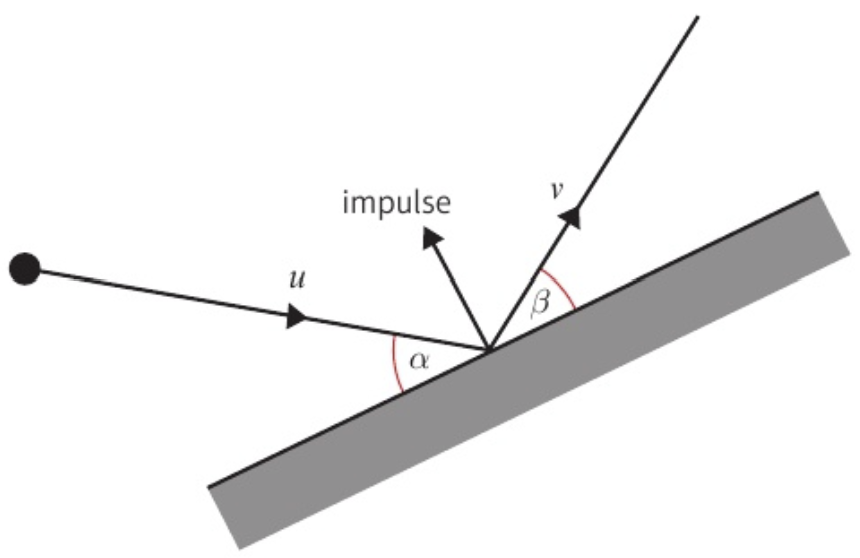
\includegraphics[width=0.3\textwidth]{obliqueimpact}
\begin{itemize}
    \item The component of the velocity of the sphere parallel to the surface is unchanged: $v\cos\beta = u\cos\alpha$
    \item The component of the velocity of the sphere perpendicular to the surface can be found with Newton's law of restitution: $v\sin\beta = eu\sin\alpha$
    \item Hence $\tan\beta = e\tan\alpha$, since $0 \leq e \leq 1$, $\beta \leq \alpha$
    \item $\text{Loss of kinetic energy}=\frac{1}{2}mu^2-\frac{1}{2}mv^2$
\end{itemize}
\section{Oblique impact of smooth spheres}
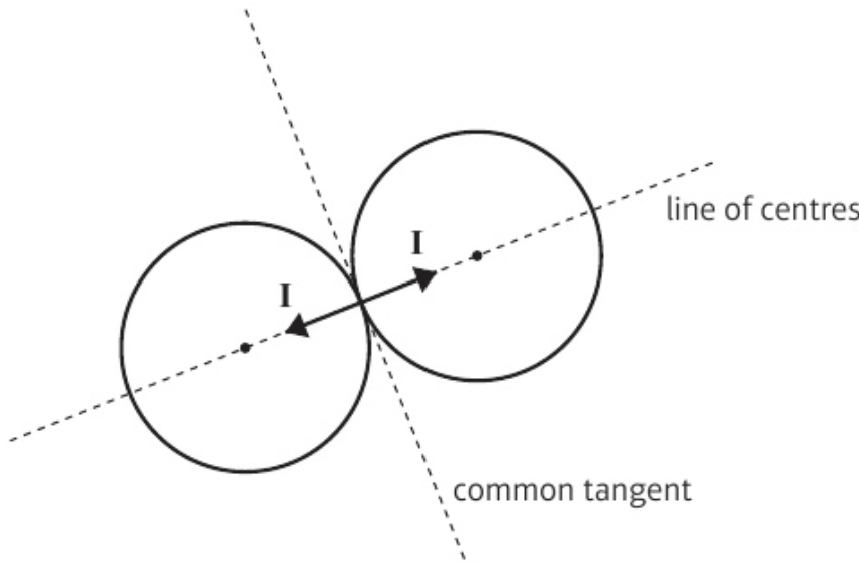
\includegraphics[width=0.3\textwidth]{oblique_2_balls}
\begin{itemize}
    \item Impulse affecting each sphere acts along the line of centres
    \item The components of the velocities of the spheres \textbf{perpendicular}  to the line of centres are unchanged in the impact
    \item The principle of conservation of momentum and Newton's law of restitution applies \textbf{parallel} to the line of centres
\end{itemize}





\end{document}